\documentclass[a4paper]{article}


\usepackage{alphabeta} 
\usepackage{enumitem} 
\usepackage{mathtools}
\usepackage{amsmath, amssymb} 
\usepackage{amsthm}
\usepackage{cancel} 
\usepackage[margin=0.70in]{geometry} 
\geometry{left=3cm,right=3cm,top=2.4cm,bottom=2.4cm}	%the page geometry as defined, A4=210x297mm
\usepackage{graphicx}
\usepackage{wrapfig}
\usepackage{caption}
\usepackage{textcomp}
\usepackage{tabto}
\usepackage{layout}
\usepackage{bm}
\usepackage{minipage-marginpar}
\usepackage[dvipsnames]{xcolor}
\usepackage{hyperref}
\usepackage{dutchcal}
\usepackage{derivative}
\usepackage{esint}
%\usepackage{biblatex}
\usepackage{subcaption}
\usepackage{booktabs}\usepackage{derivative}
\usepackage[flushleft]{threeparttable}
\usepackage[capbesideposition=outside,capbesidesep=quad]{floatrow}
\usepackage{derivative}
\usepackage[thinc]{esdiff}
%%RENEW

\newtheorem{problem}{Άσκηση}
\newtheorem*{solution*}{Λύση}
\newtheorem{definition}{Ορισμός}[subsection]
\newtheorem{properties}{Ιδιότητες}[subsection]
\newtheorem{theorem}{Θεώρημα}[subsection]
\newtheorem{protash}{Πρόταση}[subsection]
\newtheorem{porisma}{Πόρισμα}[subsection]
\newtheorem{lemma}{Λήμμα}[subsection]
\newtheorem*{prooof}{Απόδειξη}
\newtheorem*{notes}{Παρατηρήσεις}
\newtheorem*{note}{Παρατήρηση}
\newtheorem*{app}{Εφαρμογή} 
\newtheorem*{example}{Παράδειγμα}
\newtheorem*{examples}{Παραδείγματα}


\newcommand\numberthis{\addtocounter{equation}{1}\tag{\theequation}}
%\renewcommand{\labelenumi}{\roman{enumi}}
\newcommand{\approxtext}[1]{\ensuremath{\stackrel{\text{#1}}{\approx}}}
\renewcommand{\figurename}{Εικόνα.}
\renewcommand{\tablename}{Πίνακας.}
%\renewcommand\refname{New References Header}
\renewcommand*\contentsname{Περιεχόμενα}
%\DeclareDerivative{\odv}{\mathrm{d}}


\begin{document}
\begin{titlepage}			%makes a title page. Remember to change the author, CID, username and group number to what is appropriate for you!
	\centering
	{\scshape\LARGE Εθνικό Μετσόβιο Πολυτεχνείο\par}
	{\scshape \LARGE Σ.Ε.Μ.Φ.Ε.\par}
	\vspace{1cm}
	{\huge\bfseries Εξαναγκασμένες Ταλαντώσεις - Συντονισμός \par}
	\vspace{1cm}
	{\Large\itshape Θωμόπουλος Σπύρος\par}		%remember to change these!
	
	%		{\large Group \@group\unskip\strut\par}
	{\large A.M ge19042 \hfill \\}% spyros.thomop@gmail.com/ ge19042@mail.ntua.gr\par		%remember to change these!
	\vspace{1cm}
	{\large Ημερμονηνία Παράδοσης 19/11/2021\par}
\end{titlepage}


\newpage 

\subsection*{Σκοπός}
Ο στόχος της εν λόγω εργαστηριακής άσκησης είναι η μελέτη ενός κυκλώματος RLC σε σειρά. Θα χρησιμοποιήσουμε τις καμπύλες συντονισμού του ρεύματος και της διφοράς φάσης τάσης πηγής-ρεύματος συναρτήσει της συχνότητας διέγερσης. Έτσι θα προσδιορίσουμε τον συντελεστή ποιότητας, την ολική αντίσταση και τον συντελεστή αυτεπαγωγής. Ακόμη, αποσυνδέοντας την πηγή διέγερσης του κυκλώματος θα παρατηρήσουμε τις ελέυθερες φυθίνουσες ταλαντώσεις του.

\subsection*{Θεωρητικά Στοιχεία} 
%
%\begin{wrapfigure}{r}{0.4\textwidth}
%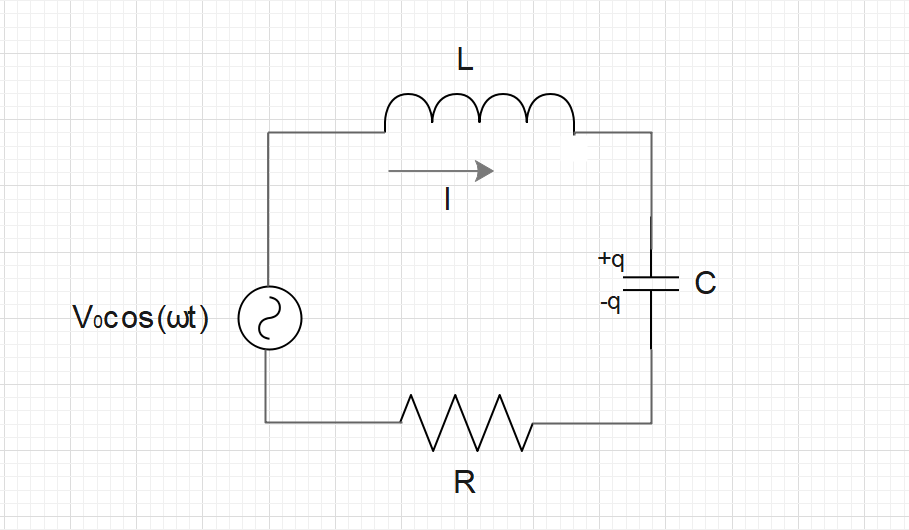
\includegraphics[width=1.0\linewidth]{circuit.png} 
%\caption{ }
%\label{fig:wrapfig}
%\end{wrapfigure}

\begin{wrapfigure}{r}{0.4\textwidth}
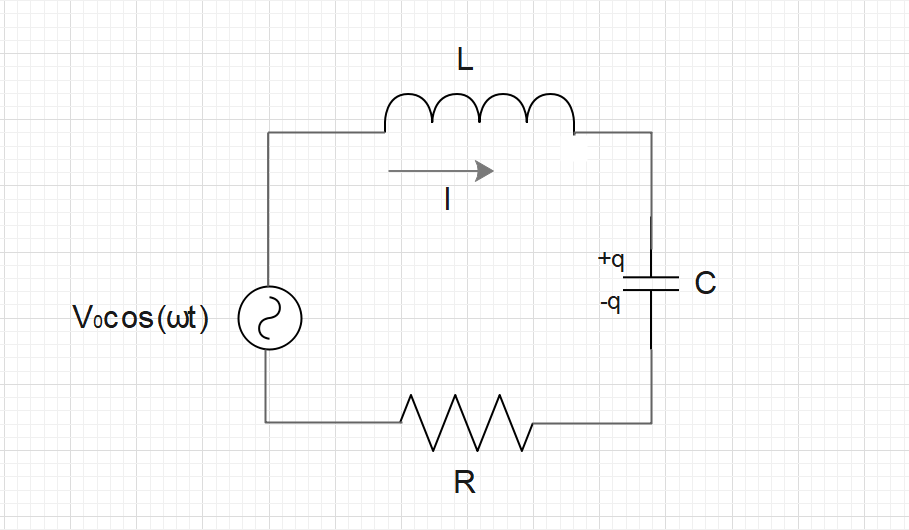
\includegraphics[width=1.0\linewidth]{circuit.png} 
\caption{ }
\label{fig:wrapfig}
\end{wrapfigure}

Η συνδεσμολογία του κυκλώματος που θα μελετήσουμε φαίνεται στην Εικόνα 1 και αποτελείεται από μία αντίσταση R, έναν πυκνωτή C, ένα πηνίο L και μια πηγή τάσης, η οποία στο κύριο μέρος του πειράματος θα δίνει περιοδική διέργερση $V_{\delta \iota\epsilon\gamma.}=V_0cos(\omega t)$. 

Αν στο κύκλωμα υπήρχαν μόνο ο πυκνωτής και το πηνίο τότε το ρεύμα θα εκτελούσε Αρμονική Ταλάντωση (μη αποσβεννύμενη), ενώ με την παρουσία της αντίστασης το πλάτος του ρεύματος θα έφθινε εκθετικά. 
Γνωρίζουμε πως αν C είναι χωρητικότητα του πυκνωτή, η τάση στα άκρα του είναι $V_C=q/ C$, ενώ η τάση πηνίο είναι 
$V_L=L\cdot \diff{I}{t}$, όπου L είναι ο συντελεστής αυτεπαγωγής. 
Ακόμη, η αντίσταση R είναι Ωμική, συνεπώς την διέπει η γραμμική σχέση $V_R=IR$.

Έτσι, απ' τον 2ο ν.Kirchhoff έχουμε ότι 
\begin{align*}\label{1}
V_C+V_R+&V_L =0 \Rightarrow \frac{q}{C}+L\diff{I}{t} +IR =0 \xRightarrow{\diff{q}{t}=I} \\ 
\diff[2]{q}{t}& +\frac{R}{L}\diff{q}{t} +\frac{1}{LC} q =0   \numberthis
\end{align*}
Ορίζουμε ως χαρακτηριστική συχνότητα του συστήματος την $\omega_0:=1/\sqrt{LC}$ και ως συντελεστή απόσβεσης $\gamma:=R/2L$. Τότε, αν έχουμε ασθενή απόσβεση, δηλαδή αν $\gamma<\omega_0$, οι λύσεις για το φορτίο q είναι της μορφής $q(t) = q_0 e^{-\gamma t} cos(\omega_0t + \phi_0)\stackrel{\text{q(0)=0}}{=}  q_0 e^{-\gamma t}sin(\omega_0t)$, παρατηρούμε δηλαδή εκθετική μείωση του πλάτους της ταλάντωσης του φορτίου, που σημαίνει απώλεια ενέργειας.
 
Για να αποφευγχθεί η παραπάνω απώλεια, θα πρέπει να πρσοθέσουμε μια εξωτερική πηγή, σκοπός της οποίας είναι να αναπληρώνει ένα μέρος της απωλεσθείσας ενέργειας σε κάθε περίοδο. Αν η πηγή είναι περιοδική με πλάτος $V_0$ και κυκλικλή συχνότητα $\omega$, τότε η εξίσωση (\ref{1}) γίνεται 
\begin{equation}\label{2}
\diff[2]{q}{t} +\frac{R}{L}\diff{q}{t} +\frac{1}{LC} q =  \frac{V_0}{L}cos(\omega t)
\end{equation}

Η λύση της παραπάνω διαφορικής εξίσωσης περνάει από μία μεταβατική φάση ύστερα από την οποία επικρατεί η επίδραση της διεγείρουσας πηγής και το ρεύμα ταλαντώνεται με την συχνότητά της:
\begin{equation}
I(t) = I_0 cos(\omega t+\phi)
\end{equation}
όπου η γωνία $\phi$ πρόκειται για την διαφορά φάσης ρεύματος κυκλώματος-τάσης πηγής. 
Άρα για τις τάσεις έχουμε:
\begin{align*}
V_R &= IR = RI_0 cos(\omega t + \phi) \numberthis \\ 
V_L &= L\diff{I}{t} = -LI_0\omega sin(\omega t + \phi) = \omega I_0 Lcos(\omega t+\phi + \pi/2) \numberthis\\ 
V_C &= \frac{q}{C} = \frac{I_0}{C\omega} sin(\omega t + \phi) =\frac{I_0}{C\omega}cos(\omega t + \phi -\pi/2)\numberthis
\end{align*} 
Παρατηρώ ότι η τάση $V_L$ προηγείται σε φάση κατά $\pi/2$ από την $V_R$ η οποία με την σειρά της προηγείται κατά $\pi/2$ από την $V_C$.

Η τάση της πηγής, ισούται με το διανυσματικό άθροισμα (σύνθεση) των τάσεων των στοιχείων του κυκλώματος, όπως φαίνεται στην Εικόνα 2.  Άρα για τα πλάτη έχουμε 
\begin{align*}\label{5}
V_1=V_L -V_C=I_0\left( \omega L - \frac{1}{C\omega}\right) \numberthis \\ 
V_0 = \sqrt{V_1^2+V_R^2} = I_0\sqrt{R^2+\left(L\omega-\frac{1}{C\omega}\right)^2} \numberthis 
\end{align*}
όπου η "σταθερά" αναλογίας μεταξύ τάσης και ρεύματος πρόκειται για την \textit{σύνθετη αντίσταση ή εμπέδηση}, $Z=\sqrt{R^2+\left(L\omega-\frac{1}{C\omega}\right)^2}$. Το πλάτος λοιπόν, του ρεύματος στην στάσιμη κατάσταση προκύπτει από την σχέση (5): 
\begin{equation}\label{9}
I_0 = \frac{V_0}{Z}
\end{equation}
Ακόμη, η διαφορά φάσης μεταξύ της τάσης της πηγής και του ρεύματος προκύπτει από την Εικόνα 2:\footnote{Το ρεύμα και η τάση στα άκρα της αντίστασης είναι συμφασικά καθώς συνδέονται από την σχέση $V_R=I  R$} 
\begin{equation}
tan\phi = \textcolor{red}{-}\frac{V_1}{V_R} = \textcolor{red}{-}\frac{\omega L - 1/C\omega}{R} \footnotemark
\end{equation}
\footnotetext{Προσθέτω ένα '-' προκειμένου όταν έχουμε μηδενική τιμή της $\omega$ να προκύπτει διαφορά φάσης 90.}
\begin{wrapfigure}{r}{0.4\textwidth}
%\begin{figure}
\centering
\caption{\centering{Διανυσματική Πρόσθεση Τάσεων}}
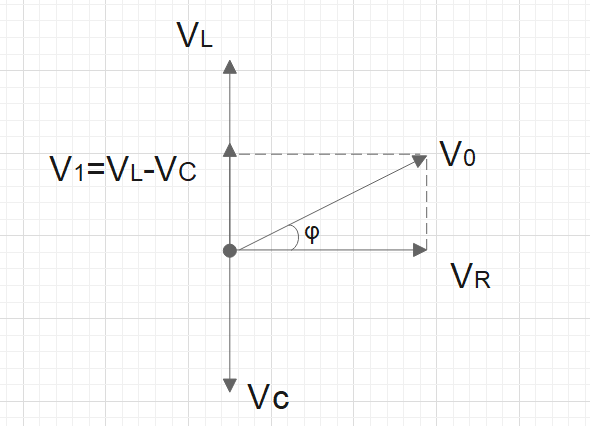
\includegraphics[scale=0.4]{coupled.png}
%\end{figure}
\end{wrapfigure}

Προφανώς, το πλάτος του ρεύματος $I_0$ είναι συνάρτηση της επιβαλλόμενης από την πηγή συχνότητας και λαμβάνει μέγιστη τιμή όταν η εμπέδηση γίνεται ελάχιστη, δηλαδή όταν
\begin{equation}\label{11}
L\omega-1/C\omega=0 \Rightarrow \omega_r=\omega_0 = \sqrt{\frac{1}{LC}}
\end{equation}
όπου η $\omega_r$ καλείται \textit{συχνότητα συντονισμού} και ισούται με την ιδιοσυχνότητα του κυκλώματος εάν αυτό αποτελούνταν μόνο απ' τα στοιχεία R,L.
 Η κατάσταση λοιπόν αυτή, κατά την οποία μεγιστοποιείται το πλάτος του ρεύματος καλείται συντονισμός του πλάτους του ρεύματος και τότε έχουμε την βέλτιστη απόκριση του κυκλώματος στην διέγερση, δηλαδή την μέγιστη προσφερόμενη ισχύ στο κύκλωμα και τον βέλτιστο τρόπο απορρόφησης της προσφερόμενης ενέργειας από το σύστημα.
  Ακόμη, στον συντονισμό μηδενίζεται η διαφορά φάσης τάσης πηγής και ρεύματος, $\phi =0$. Σε άλλες περιπτώσεις το ρεύμα προηγέιται της τάσης $(\omega>\omega_0)$ ή έπεται ($\omega<\omega_0$), αυτά φαίνονται και στην Εικόνα 4.
\begin{wrapfigure}{r}{0.4\textwidth}
%\begin{figure}
\centering
\caption{\centering{Μερικές καμπύλες συντονισμού για διαφορετικές αντιστάσεις R}}
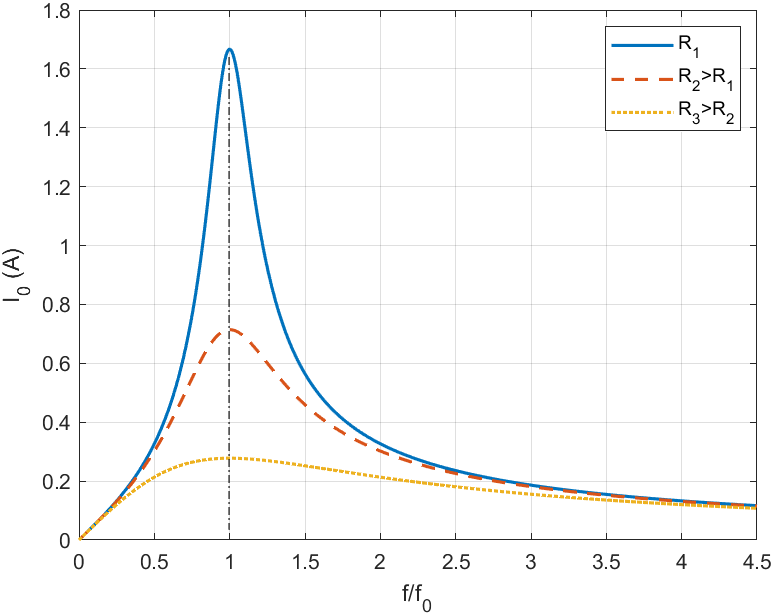
\includegraphics[scale=0.4]{rescurves.png}
%\end{figure}
\end{wrapfigure}

Όλα τα παραπάνω μπορούν να προκύψουν, έπειτα από πολλές πράξεις, αν αντικαταστήσουμε στην Διαφορική Εξίσωση (\ref{2}) την ειδική λύση για την στάσιμη κατάσταση είτε σε τριγωνομετρική μορφή $q=q_0cos(\omega t +\phi)$ είτε σε μιγαδική μορφή $q=\tilde{q_0}exp(i\omega t)$.
Κάποιες γραφικές παραστάσεις για το πλάτος του ρεύματος και για διάφορες τιμές της αντίστασης R φαίνονται στην Εικόνα 3.
\\ \\ 
Μας ενδιαφέρει να μελετήσουμε την οξύτητα της καμπύλης συντονισμού, διότι όσο πιο στενή είναι, η τιμή του ρεύματος στο κύκλωμα πλησιάζει στο μέγιστο για μικρότερη συχνοτική περιοχή, επομένως το κύκλωμα είναι καλής ποιότητας. Η αντίστοιχη καμπύλη συντονισμού για την ισχύ του κυκλώματος έχει παροόμοια μορφή με αυτή του ρεύματος. Αν για τις συχνότητες $f_1,f_2$ η τιμή της ισχύος γίνεται μισή της μέγιστης, τότε η διαφόρα των δύο συχνοτήτων ορίζεται ως \textit{Εύρος Ζώνης, $\Delta f=f_2-f_1$}. Όσο πιό μικρό το εύρος ζώνης, τόσο πιο οξεία είναι η καμπύλη συντονισμού και τότε το κύκλωμα είναι καλής ποιότητας. Οι συχνότητες $f_1,f_2$ αντιστοιχούν σε ρεύμα ίσο με $\sqrt{2}I_{0,max}/2$.
\newpage

Μπορούμε να συμπεριλάβουμε τα παραπάνω χαρακτηρηστικά σε έναν συντελεστή, τον \textit{Συντελεστή Ποιότητας Q}.

\begin{wrapfigure}{r}{0.35\textwidth}
%\begin{figure}
\centering
\caption{\centering{Διαφορά φάσης τάσης-ρεύματος για διάφορα R}}
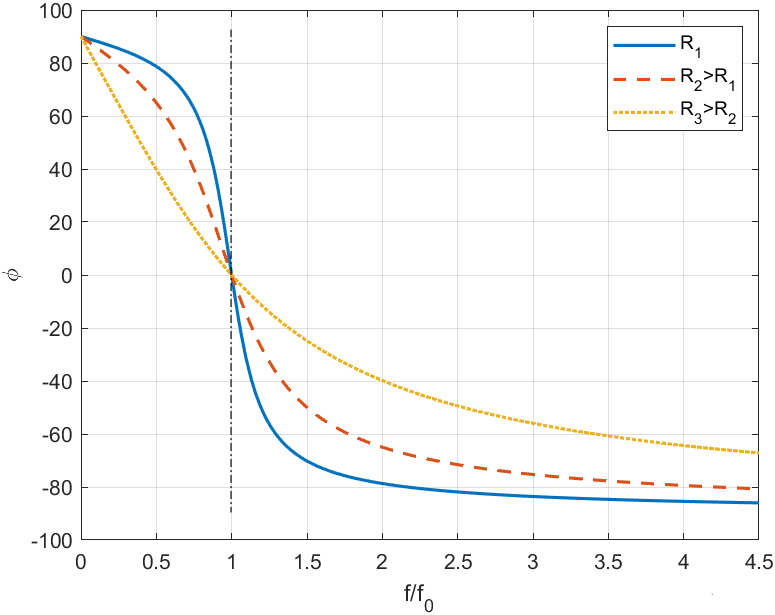
\includegraphics[scale=0.40]{phi.png}
%\end{figure}
\end{wrapfigure}
Ο ορισμός του είναι 
\begin{align*}\label{12}
Q:&=2\pi\frac{\text{Στιγμιάια Ενέργεια}}{\text{Απώλεια ενέργειας σε χρόνο Τ}}=2\pi\frac{E}{\left|\odv{E}{t}\right| T}\Rightarrow \\
&=\frac{\omega_0}{2\gamma}=\frac{\omega_0 L}{R} = \frac{\omega_0}{\Delta\omega} = \frac{f_0}{\Delta f} \numberthis
\end{align*}

Ένα τελευταίο στοιχείο του συντονισμού προκύπτει χρησιμοποιώντας τα πλάτη των τάσεων:
\begin{align*}\label{13}
\omega_0^2 = \omega_0\cdot \omega_0 &= \frac{1}{LC} \xRightarrow{(5),(6)} \frac{V_{0L}}{\cancel{I_0L}}\frac{\cancel{I_0}}{\cancel{C}V_{0C}} = \frac{1}{\cancel{LC}}\\
V_{0C} = V_{0L} & \xRightarrow{I_0=V_0/R}  V_{0L} = V_{0C} = Q V_0 \numberthis
\end{align*}


\subsection*{Πειραματική Διάταξη }
Η πειραματική διάταξη που φαίνεται στην Εικόνα 5 αποτελείται από: 
\begin{itemize}
\item[.] Γεννήτρια παλμών, χρησιμοποιείται ως πηγή αρμονικής τάσης και τετραγωνικών παλμών.
\item[.] κύκλωμα RL, τοποθετημένο πάνω σε μία βάση plexiglass, με τιμές για τα ηλεκτρικά στοιχεία $R_\mu = 100\Omega$ και $C=4.7nF$ με $\delta C =5\%$
\item[.] παλμογράφο για την μέτρηση περιόδου/πλάτους παλμών
\end{itemize}


Ο υπολογισμός της ολικής ωμικής αντίστασης από την τιμή του μεγίστου της $I_0$ περιλαμβάνει το άθροισμα της αντίστασης που φαίνεται στην Εικόνα 4 και της αντίστασης των άλλων στοιχείων του κυκλώματος - αντίσταση απωλειών $R_\alpha$, άρα $R_{ολ}=R_\mu+R_\alpha$.


\begin{figure}[h!]
\centering 
\caption{ Πειραματική Διάταξη για την μελέτη του κυκλώματος RLC }
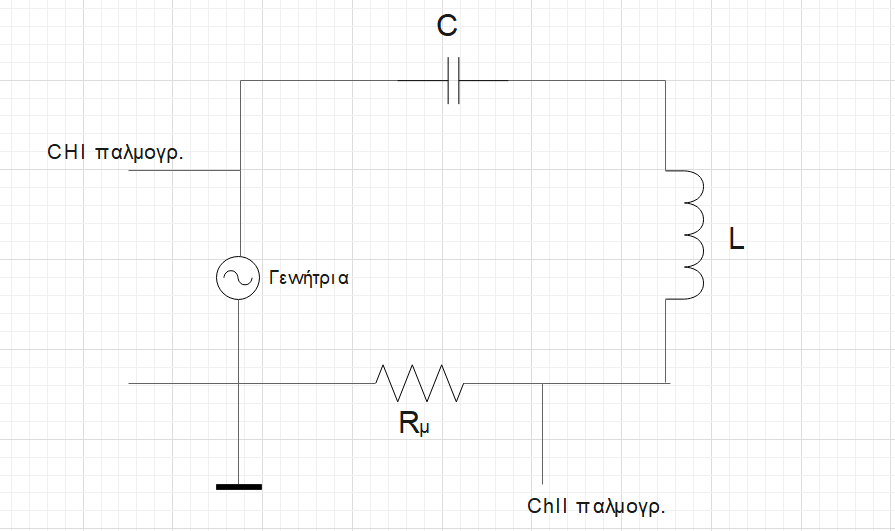
\includegraphics[scale=0.35]{circ.png}
\end{figure}


\subsection*{Πειραματική Διαδικασία - Επεξεργασία Μετρήσεων}
\subsubsection*{Καμπύλη Συντονισμού του Ρεύματος}
Πραγματοποιούμε αρχικά την συνδεσμολογία του κυκλώματος όπως φαίνεται στην Εικόνα 5. Έπειτα, από την γεννήτρια επιλέγουμε αρμονικούς παλμούς πλάτους $V_0=1V$, το οποίο προσδιορίζουμε από τον παλμογράφο και ορίζουμε την συχνότητα στο $f = 1kHz$. Για να μετρήσουμε το πλάτος της τάσης στα άκρα της αντίστασης $V_0^{\mu}$, συνδέουμε το ChII του παλμογράφου στα άκρα της. Αφήνοντας το πλάτος της τάσης αναλλοίωτο στο $V_0=(1\pm0.1)V$, αλλάζουμε την συχνότητα από $f=4-20kHz$ μετρώντας το πλάτος της τάσης για κάθε τιμή της συχνότητας. Επίσης, το ρεύμα προκύπτει από την σχέση $I_0 = V_0^{R_\mu} /R_\mu$. Τα αποτελέσματα φαίνονται στον Πίνακα 1. 
\newpage

\begin{table}
\centering 
\caption{ }
\begin{tabular}{l|l|l|l|l} 
$f_{γεν}(kHz)$  & $\#$Γραμμών & Κλιμακα\footnotemark &$V_0^{R_\mu}(V)$ & $I_0(mA)$ \\ 
\hline\hline
4.0&7.5&10mV&0.015&0.2\\ 
6.0&14.0&10&0.028&0.3\\ 
8.0&15.5&20&0.062&0.6\\ 
8.5&8.0&50&0.080&0.8\\ 
9.0&11.0&50&0.110&1.1\\ 
9.2&13.0&50&0.130&1.3\\ 
9.4&15.5&50&0.155&1.6\\ 
9.6&19.0&50&0.190&1.9\\ 
9.8&11.5&0.1V&0.230&2.3\\ 
10.0&13.5&0.1&0.270&2.7\\ 
10.3&15.5&0.1&0.310&3.1\\ 
10.4&15.0&0.1&0.300&3.0\\ 
10.6&13.5&0.1&0.270&2.7\\ 
10.8&11.5&0.1&0.230&2.3\\ 
11.0&8.5&0.11&0.170&1.7\\ 
11.5&13.0&50mV&0.130&1.3\\ 
12.0&10.0&50&0.100&1.0\\ 
14.0&5.0&50&0.050&0.5\\ 
16.0&3.5&50&0.035&0.4\\ 
18.0&6.5&20&0.026&0.3\\ 
20.0&11.0&10&0.022&0.2\\ 
\end{tabular}
\end{table}
\footnotetext{Η κλίμακα αναφέρεται σε κουτάκια, δηλαδή $V_0^{R_\mu}=\text{κλίμακα}\times\text{κουτάκια}=\text{κλίμακα}\times\text{γραμμές}/5$}

Η συχνότητα συντονισμού είναι $f_0 = (10.3\pm0.1)kHz$.

Η καμπύλη συντονισμου του ρεύματος ως συνάρτηση της συχνότητας είναι 
\begin{figure}[h!]
\centering
\caption{$I=I(f)$ }
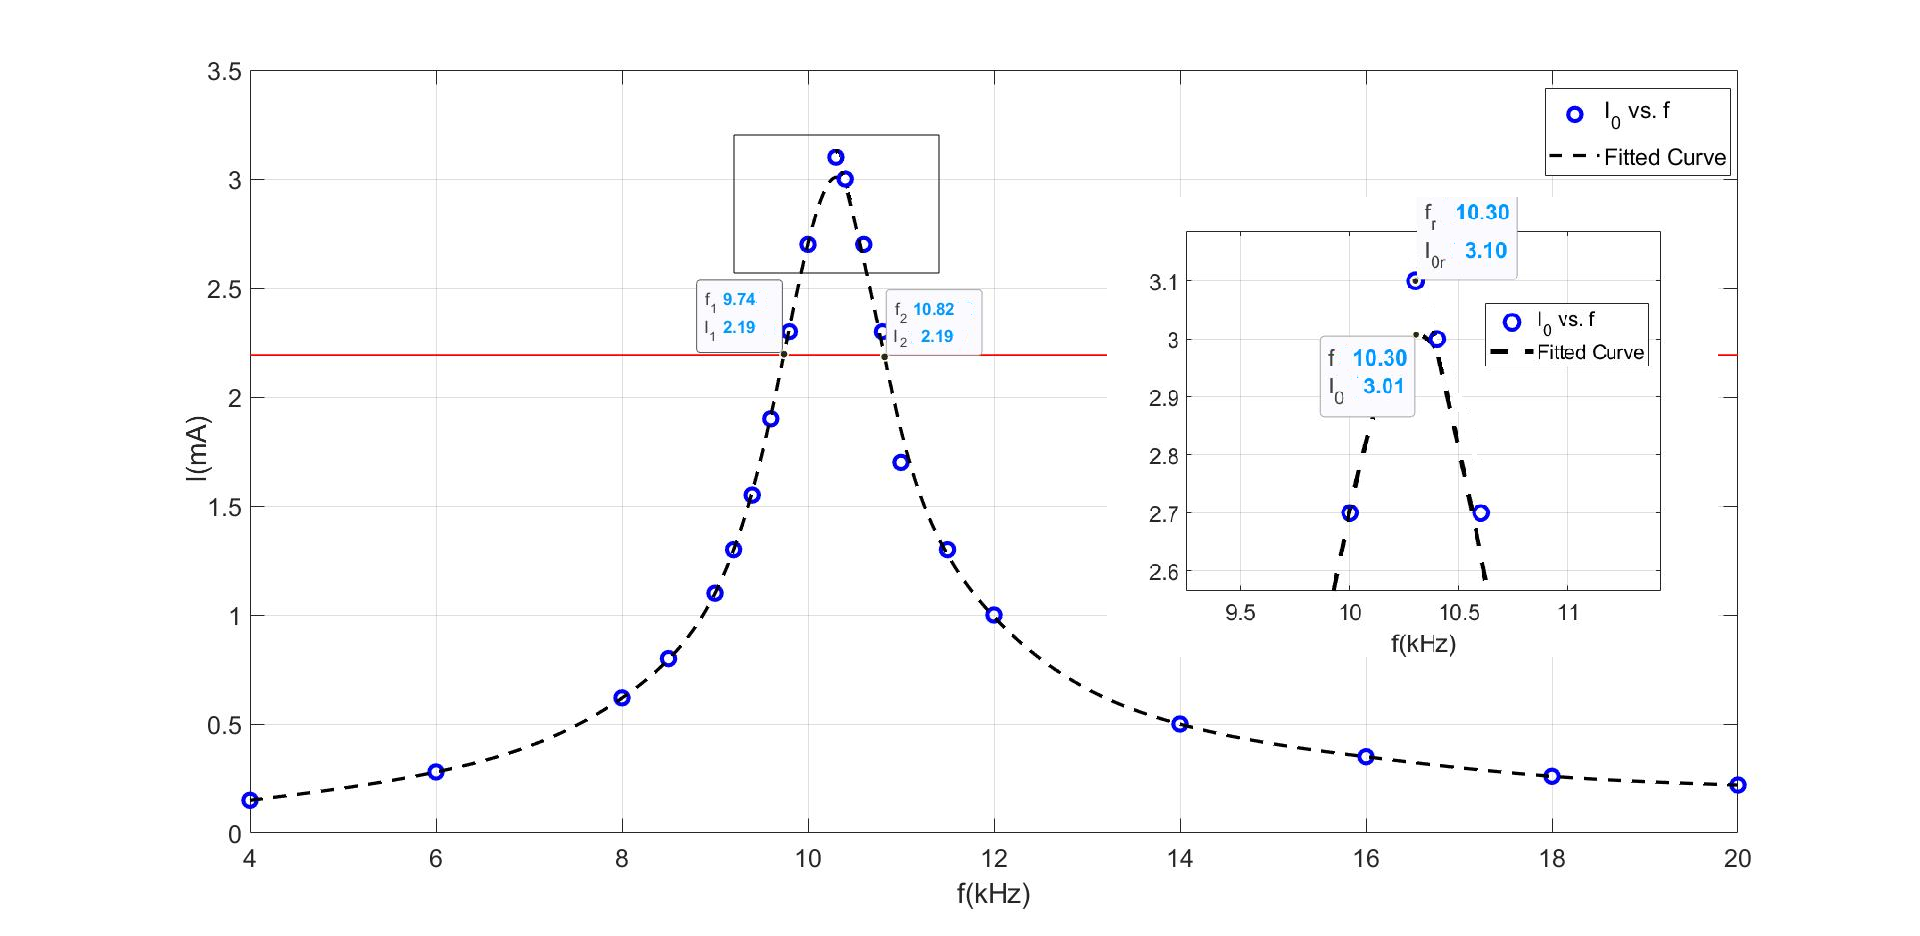
\includegraphics[scale=0.45]{I_correct.jpg}
\end{figure}

Από την γραφική προκύπτει πως η συνχότητα συντονισμού για το κύκλωμά μας είναι $$f_{0,r}=(10.3\pm 0.1 )kHz$$
Επίσης, στην γραφική παράσταση τα σημεία των οποίων φαίνονται οι συνταταγμένες, αντιστοιχούν σε τιμή του ρεύματος $\sqrt{2}I_{0,max}/2$ και έτσι προκύπτει το εύρος ζώνης 
\begin{align*}
\Delta f = (f_2-f_1)\pm \delta(\Delta f) \Rightarrow \boxed{\Delta f = ( 1.1 \pm 0.1) kHz} \footnotemark 
\end{align*}
\footnotetext{Το σφάλμα για το εύρος ζώνης προκύπτει από την διάδοση του σφάλματος των συχνοτήτων και δεδομένου ότι πρόκειται για διάδοση διαφοράς έχει τιμή $\delta(\Delta f) = \sqrt{(\delta f_1)^2+(\delta f_2)^2}=\sqrt{2}\delta f = \sqrt{2} \cdot 0.1 \simeq 0.1kHz$.}

Από την σχέση (\ref{12}) έχουμε 
\begin{align*}\label{14}
Q = \left( \frac{f_0}{\Delta f} \pm \delta Q \right)= ( 9.4 \pm 0.9)  \numberthis 
\end{align*}
'Οπου το σφάλμα του συντελεστή ποιότητας είναι 
\begin{align*}
\delta Q &= \sqrt{\left( \pdv{Q}{f_0}\delta f_0 \right)^2 + \left( \pdv{Q}{(\Delta f)} \delta(\Delta f)\right)^2 }=\sqrt{ \left( \frac{1}{\Delta f}\delta f_0 \right)^2 + \left( \frac{f_0}{(\Delta f )^2} \delta(\Delta f)\right)^2 } \Rightarrow \\ 
    & = \frac{1}{\Delta f}\sqrt{ \left( \delta f_0 \right)^2 + \left( \frac{f_0}{(\Delta f )} \delta(\Delta f)\right)^2 } \stackrel{\text{}}{=} 0.8561 \simeq 0.9
\end{align*}

Στον συντονισμό, η τιμή της εμπέδησης ισούται με την ολική αντίσταση του κυκλώματος $Z=R_{ολ.}$ και τότε, από την σχέση (\ref{9}) προκύπτει ότι $I_0 = V_0/ R_{ολ.}$. Από αυτή τη σχέση έχουμε για την ολική αντίσταση: 
\begin{align*}
R_{ολ.} = \left( \frac{V_0}{I_0} \pm \delta R_{ολ.} \right)= \left( 323 \pm 34\right) \Omega \footnotemark
\end{align*}
\footnotetext{Σφάλμα αντίστασης για $\delta V_0=0.1 V$ και $\delta I_0=0.1mA$:\\
 $\delta R_{ολ}= \sqrt{\left( \pdv{ R_{ολ}}{V_0}\delta V_0 \right)^2 + \left( \pdv{ R_{ολ}}{I_0}\delta I_0 \right)^2}=
\frac{1}{I_0}\sqrt{ \left( \delta V_0\right)^2 + \left( \frac{V_0}{(I_0 )} \delta(I_0)\right)^2 }
=33.8945\simeq 34\Omega$}

Η παραπάνω ολική αντίσταση πρόκειται για το άθροισμα της μετρητικής ανίστασης $R_\mu = 100\Omega$ και της αντίστασης απωλειών, η οποία ταυτίζεται με την αντίσταση του πηνίου $R_\alpha = R_L$, άρα $R_{ολ} = R_\mu + R_L$. Συνεπώς έχουμε 
\begin{align*}
 R_L = ( 223\pm34)\Omega 
\end{align*}
Η τιμή που προκύπτει τόσο για την ολική αντίσταση όσο και για την αντίσταση του πηνίου/απωλειών έχει πολύ μεγάλη τιμή, αφού ξεπερνάει εκείνη της μετρητικής αντίστασης.



\subsubsection*{Καμπύλη Φάσης του Ρεύματος}
Χωρίς να αλλάξουμε την συνδεσμολογία του προηγούμενου σταδίου, μεταβάλλουμε την συχνότητα πάλι από $f=4-20Hz$ και τώρα μετράμε την χρονική διαφορά, $\Delta t$, τάσης πηγής - τάσης μετρητικής αντίστασης $R_\mu$ στον οριζόντιο άξονα του παλμογράφου. Ωστόσο επειδή $V_\mu=IR_\mu$ η συμπεριφορά της τάσης και του ρεύματος της αντίστασης ταυτίζεται ως προς τον χρόνο. Άρα, η χρονική διαφορά που μετράμε ταυτίζεται με την χρονική διαφορά τάσης πηγής - ρεύματος.  Θεωρούμε $\Delta t>0$ όταν η τάση έπεται του ρεύματος, ενω $\Delta t<0$ όταν προηγείται. Επίσης η πειραμετική τιμή της διαφοράς φάσης φ, προκεύπτει απ' την σχέση $\phi_{exp.} = 2\pi f\Delta t $.
Τα αποτελέσματα φαίνονται στον Πίνακα 2.

Πρέπει να σημειωθεί ακόμη ότι η συχνότητα συντονισμού, δηλαδή η συχνότητα για την οποία είχαμε $\phi=0$ βρέθηκε και πάλι $f_0 = (10.3\pm 0.1)Hz$ και ότι οι πειραματικές τιμές για την διαφορά φάσης προκύπτουν από την σχέση $\phi_{exp.}=(2\pi f\Delta t)  rad=(360f\Delta t)deg$.
\\ \\
Από τις τιμές του Πίνακα 2 προκύπτει η παρακάτω καμπύλη της πειραματικής διαφοράς φάσης, $\phi_{exp}$, συναρτήσει του λόγου συχνοτήτων $f/f_0$. Προκειμένου να προκύψει τόσο ομαλή όσο φαίνεται, κατά την προσαρμογή της στα πειραματικά σημεία δεν έχω λάβει υπόψιν εκείνα που σημειώνονται με κόκκινο 'x'.


\newpage

\begin{table}[h!]
\centering
\caption{ }
\begin{tabular}{r|r|r|r|r|r}
$f(kHz)$ & Γραμμές & Κλίμακα$(\mu s)$ & $\Delta t (\mu s)$ & $f/f_0$ & $\phi_{exp.} (^\circ)$ \\
\hline\hline 
4.0&3.0&100.0&60.0&0.39&86.40\\ 
6.0&2.0&100.0&40.0&0.58&86.40\\ 
8.0&3.0&50.0&30.0&0.78&86.40\\ 
8.5&2.5&50.0&25.0&0.83&76.50\\ 
9.0&2.0&50.0&20.0&0.87&64.80\\ 
9.5&4.0&20.0&16.0&0.92&54.72\\ 
10.0&3.0&20.0&12.0&0.97 &43.20\\ 
10.5&-4.0&10.0&-8.0&1.02&-30.24\\ 
11.0&-3.5&20.0&-14.0&1.07&-55.44\\ 
11.5&-4.0&20.0&-16.0&1.12&-66.24\\ 
12.0&-4.0&20.0&-16.0&1.17&-69.12\\ 
14.0&-4.0&20.0&-16.0&1.36&-80.64\\ 
16.0&-4.0&20.0&-16.0&1.55&-92.16\\ 
18.0&-3.0&20.0&-12.0&1.75&-77.76\\ 
20.0&-3.0&20.0&-12.0&1.94&-86.40
\end{tabular}
\end{table}


\begin{figure}[h!]
\centering 
\caption{Πειραματική Καμπύλη $\phi-f/f_0$.  Κατά τον σχεδιασμό της έχουν παραληφθεί τα πειραματικά \text{\hspace{0.58in}} σημεία που είναι σημειωμένα με κόκκινο. }
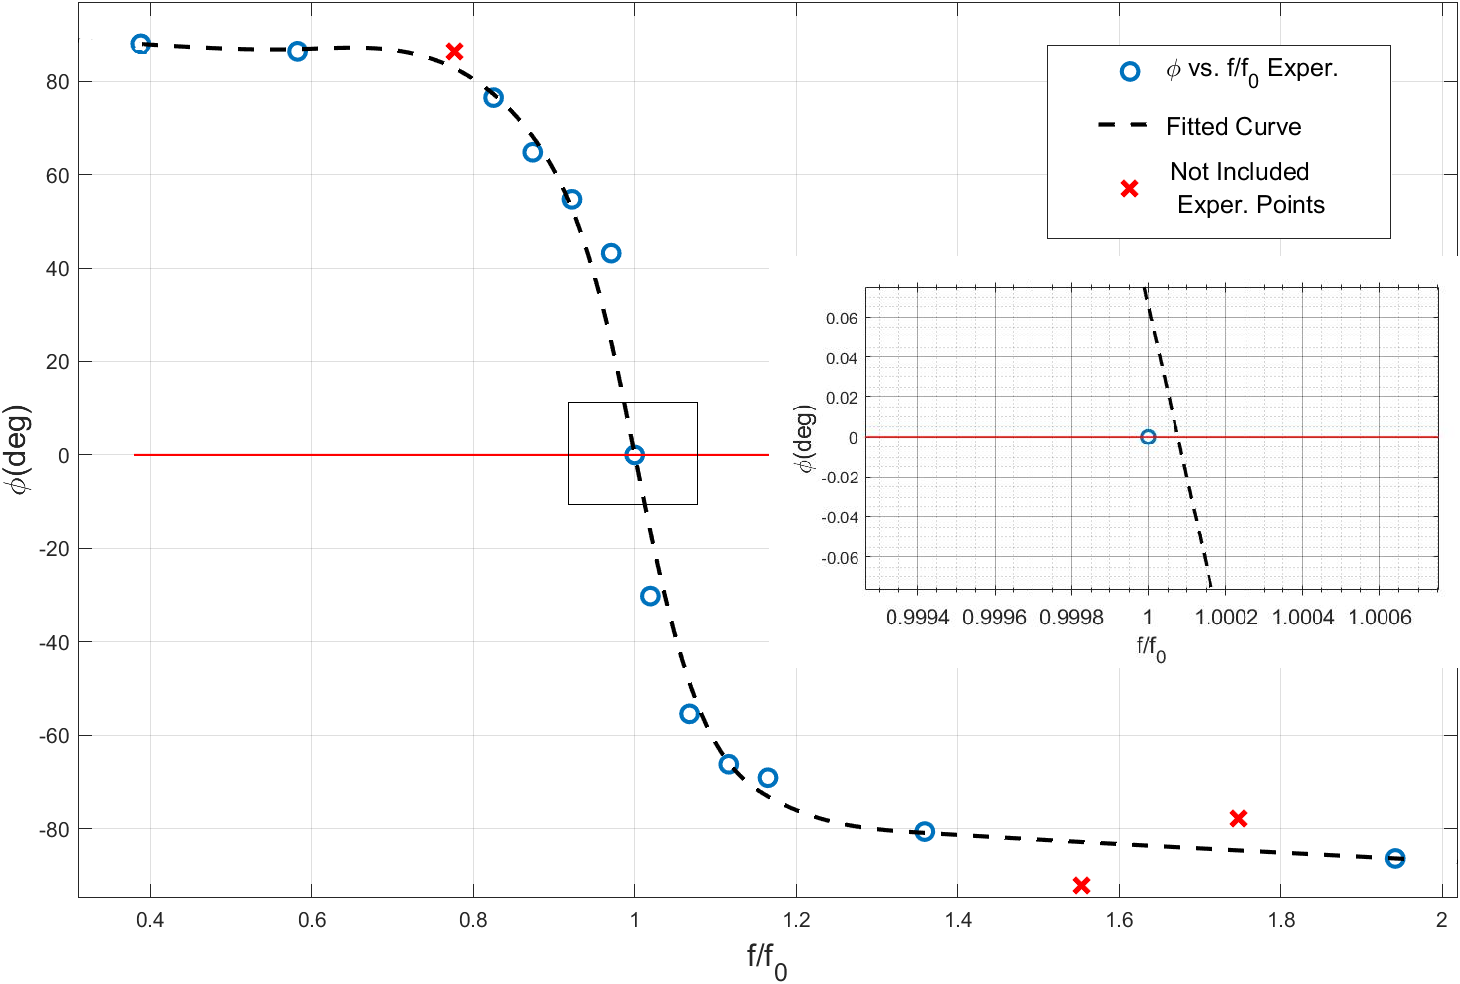
\includegraphics[scale=0.6]{phi_data.png}
\end{figure}

Παρατηρούμε ότι η πειραματική καμπύλη περνάει πρακτικά από το σημείο (1,0) όπως περιμένουμε θεωρητικά. Η απόκλισή της από το εν λόγω σημείο είναι $\sim 0.0001$ στον άξονα $f/f_0$, απόκλιση η οποία είναι εμφανώς στο πλαίσια του σφάλματος και μάλιστα θεωρείται αμελητέα.
Επιπλέον η φάση γίνεται αρνητική μετά τον μηδενισμό, δηλαδή το ρεύμα στο κύκλωμα προηγείται σε φάση από την τάση του διεγέρτη-πηγή, επιβεβαιώνοντας έτσι την θεωρία.

Ωστόσο, επειδή υπάρχουν και άλλοι τρόποι να προσαρμοστεί η καμπύλη στα πειραματικά δεδομένα, οι οποίοι ενδέχεται να μην δίνουν τόσο μικρό σφάλμα, θα θεωρήσω το σφάλμα της συχνότητας συντονισμού που προκύπτει από την καμπύλη $\delta (f_{0,\phi}/f_0) = 0.01 \Rightarrow \delta f = 0.1$
Άρα από την πειραματική καμπύλη φάσης, η συχνότητα συντονισμού προκύπτει
\begin{equation}\label{15}
f_{0,\phi} = ( 10.3 \pm 0.1 ) kHz
\end{equation}
 


Για την συχνότητα συντονισμού από την σχέση (\ref{11}) έχουμε για την αυτεπαγωγή: $L=1/4\pi^2 C f_{0,\phi}^2 = 0.0508H$. Άρα το σφάλμα της έιναι 
\begin{align*}
\delta L &= \sqrt{\left( \pdv{L}{C}\delta C \right)^2 + \left( \pdv{L}{f_{0,\phi}}\delta f_{0,\phi} \right)^2} =
  	 \frac{1}{4\pi^2}\sqrt{\left( \frac{1}{C^2 f_{0,\phi}^2}\delta C \right)^2+ \left( \frac{2}{Cf_{0,\phi}^3}\delta f_{0,\phi}\right)^2} \xRightarrow{C=4.7nF,\delta C =5\%C\simeq 0.235nF}   \\ 
  	 &= 0.0027248\simeq 0.003 H
\end{align*}
Δηλαδή, \vspace{-0.23in}
\begin{align*}\label{16}
L = ( 0.051\pm0.003) H \numberthis
\end{align*}


Τέλος από την σχέση (\ref{12}) προκύπτει ότι $R_{ολ}=2\pi f_0L/Q = 351.244\Omega$ καθώς έχει ήδη προσδιορισθεί ο συντελεστής ποιότητας του κυκλώματος (Σχέση (\ref{14})). Άρα 
\begin{align*}
R_{ολ} = ( 351\pm 39) \Omega
\end{align*}
με το σφάλμα να δίνεται από την
\begin{align*}
\delta R_{ολ}& = \sqrt{\left( \pdv{R_{ολ}}{Q} \delta Q \right)^2 + \left( \pdv{R_{ολ}}{f_0}\delta f_0\right)^2+\left( \pdv{R_{ολ}}{L}\delta L \right)^2 }=
		2\pi\sqrt{ \left( \frac{f_0L}{Q^2} \delta Q\right)^2 + \left( \frac{L}{Q}\delta f_0\right)^2 +\left( \frac{ f_0}{Q}\delta L 						\right)^2}   \xRightarrow{(\ref{14}),(\ref{15}),(\ref{16})}\\
		& = 38.822992 \simeq 39 \Omega
\end{align*}


Με αυτή την μέθοδο για τον υπολογισμό της $R_{ολ}$ προκύπτει σχετικό σφάλμα $\sim 11.1\%$ ενω με την προηγούμενη ελαφρώς μικρότερο $\sim 10.5\%$. Σε πρώτη σκέψη αυτό φαίνεται λογικό καθώς στο σφάλμα της $R_{ολ}$ με την πρώτη μέθοδο υπεισέρχονται λιγότεροι όροι οι οποίοι διαδίδουν το σφάλμα τους, συνεπώς θεωρώ πως η πρώτη μέθοδος είναι προτιμητέα.

\subsubsection*{Παρατήρηση Ελεύθερων Ταλαντώσεων}

Επιλέγουμε στην γεννήτρια να παράγει ορθογώνιους παλμούς με συχνότητα $f=0.2kHz$. Αυτό που παρατηρούμε είναι ότι η ένταση του ρεύματος που ανιχνεύει ο παλμογράφος φθίνει εκθετικά. Για την μικρή συνχότητα που έχουμε επιλέξει φαίνεται ότι η ένταση προλαβαίνει να μηδενιστεί μέχρι να εκπεμφθεί από την γεννήτρια ο επόμενος παλμός, γεγονός που το αντιλαμβανόμαστε με την μεγιστοποίηση της έντασης  του ρεύματος. Ακόμη, αυξάνουμε την συχνότητα της παραγωγής παλμών και πλέον, παρόλο που διατηρείται η εκθετική μείωση, το ρεύμα δεν προλαβαίνει να μηδενιστεί πρωτού το ενισχύσει η γεννητρια με νέο παλμό.

\subsection*{Συμπεράσματα}

Τα συμπεράσματα είναι θετικά καθώς σε πρώτο επίπεδο έχουν επιβεβαωθεί ποιοτικά όλα τα θεωρητικώς αναμενόμενα στοιχεία και κυρίως προέκυψαν σωστές μορφές για τις καμπύλες συντονισμού και διαφοράς φάσης. Ακόμη, η συχνότητα συντονισμού βρέθηκε ίδια (!;) με όλες τις μεθόδους. 

\subsection*{Βιβλιογραφία}
\begin{itemize}
\item[.] ΕΡΓΑΣΤΗΡΙΑΚΕΣ ΑΣΚΗΣΕΙς ΦΥΣΙΚΗΣ ΤΟΜΟΣ ΙΙ, ΣΥΛΛΟΓΙΚΟ
\item[.]  Η Φυσική των Ταλαντώσεων και των Κυμάτων, Pain H.John
\end{itemize}


\end{document}
